\documentclass[12pt,a4paper]{article}

%%Packages and settings I use in most documents.
\usepackage[spanish]{babel}
\usepackage{ucs}
\usepackage[utf8x]{inputenc}
%\usepackage[T1]{fontenc} %Produce una salida llena de caracteres raros
\usepackage{xcolor}
\usepackage{fancyvrb}

\usepackage[section]{placeins}

\usepackage{amsmath,amsfonts}
\usepackage{graphicx}
\usepackage[space]{grffile} %% Para incluir archivos con espacios
\usepackage{hyperref}
\hypersetup{
    colorlinks=false,
    citecolor=black,
    filecolor=black,
    linkcolor=black,
    urlcolor=black,
    linkbordercolor=gray
}
\usepackage[all]{hypcap}    %for going to the top of an image when a figure reference is clicked

\usepackage{fancyhdr} 	%%Para encabezados

\usepackage{parcolumns}
\usepackage{listings}
\lstset{
  literate={ö}{{\"o}}1
           {ä}{{\"a}}1
           {ü}{{\"u}}1
           {á}{{\'a}}1
           {Á}{{\'A}}1
           {é}{{\'e}}1
           {É}{{\'E}}1
           {í}{{\'i}}1
           {Í}{{\'I}}1
           {ó}{{\'o}}1
           {Ó}{{\'O}}1
           {ú}{{\'u}}1
           {Ú}{{\'U}}1
           {ñ}{{\~{n}}}1
           {Ñ}{{\~{N}}}1
           {ç}{{\c{c}}}1
           {Ç}{{\c{C}}}1
}
\usepackage{tcolorbox} %%para utilizar cajas que no se quedan abiertas en los listings
\tcbuselibrary{listings,skins,breakable}
\newtcblisting{mycode}{
      arc=0mm,
      top=0mm,
      bottom=0mm,
      left=3mm,
      right=0mm,
      width=\textwidth,
      boxrule=1pt,
      colback=blue!10,
      listing only,
      listing options={style=mystyle},
      breakable
}
%% Mi propio tcb input
\newcommand{\mytcbinputlisting}[1]
{
  \tcbinputlisting{  
    listing file=#1,
    arc=0mm,
    top=0mm,
    bottom=0mm,
    left=3mm,
    right=0mm,
    width=\textwidth,
    boxrule=1pt,
    colback=blue!10,
    listing only,
    listing options={style=mystyle},
    breakable
  }
}
\lstdefinestyle{mystyle}{
  language=C,
  basicstyle=\footnotesize\ttfamily,
  keywordstyle=\color{blue},
  stringstyle=\color{red},
  commentstyle=\color{black!75},
  directivestyle={\color{magenta}},
  breakatwhitespace=false,
  showstringspaces = false,
  numbers = left,
  numbersep = 15pt,
  numberstyle = \footnotesize,
  stepnumber=5,
  breaklines=true,
  tabsize=2
}

\textheight=22.94cm \textwidth=17cm \topmargin=-1cm
\oddsidemargin=-0.4cm
\parindent=1.0cm

%Para permitir figuras más a menudo:
\renewcommand{\topfraction}{.85}
\renewcommand{\bottomfraction}{.7}
\renewcommand{\textfraction}{.15}
\renewcommand{\floatpagefraction}{.66}
\renewcommand{\dbltopfraction}{.66}
\renewcommand{\dblfloatpagefraction}{.66}
\setcounter{topnumber}{9}
\setcounter{bottomnumber}{9}
\setcounter{totalnumber}{20}
\setcounter{dbltopnumber}{9}

\setlength{\parskip}{\baselineskip} %Esto se utiliza para echarle cuenta a los intros

\newcommand{\encabezados}[2]{
  \pagestyle{fancy}
  \renewcommand{\headrulewidth}{0.4pt}
  \renewcommand{\footrulewidth}{0.0pt}
  \fancyhf{}
  \fancyhead[LO]{\leftmark}
  \fancyhead[RE]{\rightmark}
  \fancyhead[CE]{}
  \fancyhead[RO]{#1}
  \fancyfoot[RO]{\thepage}
  \fancyfoot[LO]{#2}
}

% Para guardar el número de un enumerate y continuar después
% \newcounter{saveenumi}
% \newcommand{\savecounteri}{\setcounter{saveenumi}{\value{enumi}}}
% \newcommand{\restorecounteri}{\setcounter{enumi}{\value{saveenumi}}}

%%%%%%%%%%%%%%%%%%%%%%%%%%%%%%
%% Definición de la Portada %%
%%%%%%%%%%%%%%%%%%%%%%%%%%%%%%
%%PARÁMETROS
%%1: Nombre de la Asignatura
%%2: Nombre del Profesor
%%3: Curso
%%4: Título
%%5: Subtítulo
\newcommand{\portada}[5]{
\begin{titlepage}
  \begin{tabular}{l}
    \sc Universidad de Murcia \\
    \sc Facultad de Informática \\
	\sc #1\\
	\sc #2\\
	\sc #3
  \vspace*{1.9cm}\mbox{}
  \end{tabular}
  \bigskip

  \vspace*{0.5 cm}
  \begin{center}
  \textbf{\Huge #4 } \\ [1.0cm]
  \textbf{\Large #5}\\
  \end{center}
  \vspace*{9 cm}
  \begin{flushright}
    \begin{tabular}{ll}
		Juan José Andreu Blázquez\\ $<$juanjose.andreu@um.es$>$ \\
         \today \\
    \end{tabular}
  \end{flushright}
\end{titlepage}
}



\begin{document}
\portada{Diseño y Estructura Interna de un SO}{Juan Piernas, Diego Sevilla}{5º de Ingeniería Informática}{Dedupfs\\\vspace{0.4cm} Sistema de ficheros con deduplicación basado en FUSE}{Convocatoria de Junio, curso 2014-2015}

\tableofcontents
\newpage
\section{Resumen del trabajo realizado}

El objetivo de este proyecto de programación práctico ha sido desarrollar un sistema de ficheros con FUSE capaz de detectar cuándo se almacenan ficheros idénticos, y dejar solo una copia de los datos en el sistema de ficheros, haciendo que el resto de ficheros sean simples apuntadores a la copia que contiene los datos. Esto permite que, en sistemas de ficheros donde hay muchos ficheros iguales, se ahorre una cantidad importante de espacio en disco.

Esta deduplicación de ficheros idénticos, se hace de forma transparente al usuario del sistema de ficheros, por lo que se siguen viendo ambos archivos como archivos diferentes, y en caso de modificarse uno de ellos, se volverán a separar y quedarán como dos ficheros diferentes. El usuario no llega a percibir estos cambios, y él utiliza su sistema de ficheros de forma normal, pero se ahorra espacio si tiene muchos archivos iguales.
Para detectar si dos ficheros son idénticos, se ha utilizado la función SHA1 para calcular la clave de dispersión del archivo. Con esta clave se almacenan los datos en un directorio del sf, con un fichero que tiene como nombre el código hexadecimal del hash, y se deja el fichero original vacío como un marcador. En una base de datos interna, se almacenan una relación de cada nombre de fichero y qué clave de dispersión le corresponde, además de algunos parámetros adicionales que se indican más adelante. Esto permite saber dónde se encuentran realmente los datos de cada fichero, y se pueden mover fácilmente de un lugar a otro cuando se modifican y se recalcula su clave de dispersión.

El cálculo de la clave de dispersión es algo costoso, puesto que implica leer el fichero completo, y realizar cálculos sobre los datos del fichero para obtener la clave. Debido a esto, es necesario buscar el momento más adecuado para calcular la clave y evitar un impacto considerable sobre la velocidad del sistema de ficheros. Este momento adecuado se produce cuando un archivo ha sido abierto para escribir en él por uno o más procesos, se ha escrito en él, y lo cierra el último de los procesos que lo tenía abierto. Entonces se recalcula la clave de dispersión y, si ésta ha cambiado, se mueven los datos al fichero que corresponda a esa clave.

Además del deduplicado de archivos, también es necesario asegurarse de que otro tipo de funcionalidades típicas de un SF en UNIX están correctamente implementadas. Para asegurar que el funcionamiento de los enlaces físicos permanece intacto en nuestro SF, se ha utilizado una tabla adicional en la base de datos que almacena para cada enlace, cuál es el archivo que posee los contenidos. En cuanto a los enlaces simbólicos, no es necesario llevar a cabo ninguna acción especial para que funcionen de forma normal.

Por último, los permisos y el resto de atributos que tiene un archivo, se almacenan en el archivo vacío que se deja de marcador, a excepción del tamaño de archivo, que también se almacena en la base de datos junto a cada archivo para facilitar el acceso posterior a esta información.

\newpage
\section{Glosario de conceptos}

A lo largo de esta memoria explicativa del desarrollo de la práctica propuesta, se utilizan una serie de términos cuyo significado se explica a continuación:
\begin{itemize}
 \item \textbf{Hash/Clave de dispersión}: Clave de 20 bytes generada a partir de un archivo mediante la función criptográfica SHA1 y que se utiliza como identificador del contenido de un archivo.
 \item \textbf{Deduplicar/deduplicado}: Cuando se habla de deduplicar un archivo, o de uno deduplicado, se hace referencia a la acción de coger dos archivos idénticos que están duplicados en el sf, y dejar solo uno conteniendo los datos.
 \item \textbf{Marcador}: Un marcador es el archivo vacío con el nombre original que se deja en el lugar donde se creó un fichero en primer lugar.
 \item \textbf{Archivo de datos}: Archivo que se crea en una carpeta oculta del sistema de ficheros y que contiene los datos a los que apuntan los marcadores. Su nombre se corresponde con el hash generado por los datos contenidos en él.
 \item \textbf{Reduplicar}: Este término se refiere a un archivo que se vuelve a duplicar cuando estaba deduplicado, porque sus contenidos han cambiado.
 \item \textbf{Punto de montaje}: Es el punto del árbol de ficheros en el que se monta el sistema de ficheros dedupfs, y desde donde se interactúa con él. En este directorio no se almacena información, si no que sirve de lugar de acceso a los datos.
 \item \textbf{Directorio subyacente/raíz}: Corresponde con el subárbol de ficheros donde se almacenan realmente los datos del sistema de ficheros dedupfs. Si se accede a los datos a través de este directorio, en puesto de a través del punto de montaje, sólo se verán los marcadores vacíos, y no se podrá acceder a sus datos.
\end{itemize}


\newpage
\section{Descripción del sistema de ficheros}

El diseño e implementación del sistema de ficheros \emph{Dedupfs} se ha llevado a cabo teniendo en cuenta desde el primer momento cuáles eran los principales retos a tener en cuenta para lograr la deduplicación totalmente transparente al usuario.
\begin{itemize}
 \item Es necesario conocer qué ficheros están deduplicados y cuáles no, y dónde se encuentran sus datos, para ello se utiliza una base de datos sqlite que se almacena en la dirección \texttt{\small .dedupfs/dedupfs.db}.
 \item Es necesario que los archivos deduplicados permanezcan independientes de cara al usuario del sistema de ficheros, y que los camios producidos en uno de ellos no se propaguen a otros. Además, sus permisos, tiempos de modificación, y otros atributos, deben permanecer independientes. Por este motivo se ha optado por dejar un marcador vacío en el lugar de cada archivo, donde se conservan sus permisos y otros atributos, y almacenar los datos en una subcarpeta del directorio \texttt{\small .dedupfs/data/} con el hash de los datos como nombre de archivo.
 \item Los enlaces físicos sirven para designar al mismo fichero con diferentes nombres desde el punto de vista del usuario. Es necesario tratarlo de la forma adecuada, y evita tratar enlaces físicos como si fueran archivos deduplicados. Para ello se ha creado una segunda tabla en la base de datos, que contabiliza estos enlaces y permite gestionar los archivos.
 \item Para evitar realizar el cálculo de hash cuando un archivo todavía puede ser modificado, lo más adecuado es hacerlo solamente cuando un fichero haya sido modificado, y deja de ser utilizado. Para ello se almacena en memoria un mapa de archivos abiertos para escritura, se marca si son modificados, y se computa su hash cuando los cierra el último proceso que los tenga abiertos.
\end{itemize}

Todo lo anterior se ha implementado modificando las funciones principales del ejemplo \texttt{\small bbfs.c}, copiándolas en otro llamado \texttt{\small dedupfs.c}, y añadiendo algunas nuevas.

También, se ha incluido un módulo llamado \texttt{\small database} que se encarga de gestionar toda la comunicación del módulo principal con las distintas tablas de la base de datos y con el mapa de ficheros abiertos (que también ha sido implementado como una base de datos sqlite en memoria).

Se ha mantenido y utilizado, por conveniencia, el módulo \texttt{\small log} para servir de ayuda en la depuración durante el desarrollo del programa. Aunque se ha definido un flag del preprocesador que anula el uso de este sistema de log una vez que el programa ha sido finalizado, puesto que el flujo de informaciónn generado por éste era demasiado alto.

Finalmente, se ha ampliado el fichero de cabecera \texttt{\small params.h} con la definición de algunas estructuras de datos, y la inclusión de cabeceras nuevas que han sido necesarias.

\subsection{Estructuras de datos}

Como se ha indicado en el apartado anterior, las estructuras de datos utilizadas en el proyecto se han basado en bases de datos sqlite3, tanto para el almacenamiento de la información de archivos deduplicados y sus hashes, como para el mapa de archivos abiertos en memoria. Incluyendo también los enlaces físicos.

\begin{itemize}
 \item \textbf{Base de datos de archivos}: La base de datos de archivos está formada por dos tablas, y se almacena en \texttt{\small .dedupfs/dedupfs.db} dentro del directorio subyacente. La primera tabla, la tabla de archivos \emph{(files)}, contiene una entrada por cada archivo de datos almacenado en nuestro SF. En dicha entrada se almacena la siguiente información:
  \begin{itemize}
    \item Path: El path del archivo lógico. Que se dejará como marcador.
    \item Shasum: El hash SHA1 de los datos del archivo, almacenado en texto con representación hexadecimal.
    \item Datapath: El path donde se almacenan físicamente los datos del archivo en el SF.
    \item Size: El tamaño en bytes del archivo, para acceder a esta información cómodamente, puesto que no está disponible en le marcador.
    \item Deduplicados: La cuenta de veces que están deduplicados los datos del archivo, empieza en 0 para archivos no deduplicados.
  \end{itemize}
  Con esta información se pueden realizar fácilmente todas las operaciones necesarias para deduplicar y reduplicar los archivos, y saber en qué estado está cada uno en cada momento.\\
  
  En esta base de datos de datos también se guarda la tabla de enlaces físicos, llamada \emph{links}. En ella se guarda para cada enlace físico, cuál es el archivo que se debe buscar en la tabla de archivos para encontrar sus datos.
    \begin{itemize}
    \item Linkpath: El path del enlace físico.
    \item Originalpath: El path del archivo cuya entrada de la tabla de archivos posee toda la información.
  \end{itemize}
  
  \item \textbf{Mapa de ficheros abiertos}: En esta estructura se guarda qué archivos han sido abiertos para escritura, de forma que se pueda saber cuando se cierran, si han sido modificados y si es el último descriptor siendo cerrado de ese archivo. Este mapa se ha establecido como una base de datos sqlite residente en memoria, ya que solo es necesario durante la ejecución del SF. Cada entrada de la tabla contiene la siguiente información:
  \begin{itemize}
   \item fh: Descriptor de ficheros utilizado para abrir este archivo.
   \item path: Path del archivo lógico que está abierto para escritura.
   \item deduplicado: Si el archivo está deduplicado o no.
   \item modificado: Indicador de si el archivo ha sido modificado o no. Un archivo puede abrirse para escritura, y finalmente no ser modificado.
  \end{itemize}
\end{itemize}

Con estas tres tablas, dedupfs tiene toda la información necesaria de cada archivo para realizar cualquier operación que se le solicite.

En el fichero de cabecera \texttt{\small param.h} se han incluido dos \emph{struct} que se corresponden con las entradas en la base de de datos de archivos, y en el mapa de ficheros abiertos en escritura.

\subsection{Implementación de la funcionalidad}

La funcionalidad completa del sistema de ficheros dedupfs dista bastante de ser trivial en muchas de las funciones que ha habido que reimplementar. Para explicar el funcionamiento de las nuevas funciones implementadas, vamos a seguir el flujo de ejeución, explicando cada una de las partes implicadas en él.

\subsubsection{Apertura, lectura, escritura, y cierre de un fichero}

Estas cuatro operaciones componen la funcionalidad fundamental del sistema de ficheros. Pasamos a explicar el comportamiento de dedupfs en estas operaciones.

\paragraph{Apertura:}
Cuando se produce la apertura de un archivo, dedupfs recibe una llamada a la función \textbf{bb\_open} con el path del archivo, y los indicadores de apertura correspondientes. Lo primero que hace el SF en este caso, es comprobar que puede abrir el marcador. Si no hay ningún problema al acceder al marcador, entonces se abre el archivo de datos: Se mira si es un enlace duro, y de serlo, se obtiene el archivo al que apunta. Tras esto, se busca este archivo en la base de datos. En caso de estar en la bd, se coge el path de su archivo de datos. Si está deduplicado y se abre en escritura, es necesario abrir una copia, para evitar contaminar el archivo de datos deduplicado (se realiza esta copia si es el primer open de este archivo), esta copia se llama idéntica al archivo de datos, sólo que añadiendo una 'w' al final.
Si no estuviera en la base de datos, simplemente se utilizará el marcador.
Finalmente se abre el path que corresponda, y una vez abierto y si se hace en escritura, se introduce en el mapa de archivos abiertos para escritura.

La creación de un archivo nuevo puede verse como un caso particular de apertura en el que se abre un archivo nuevo para escribir en él. En este caso, cuando se recibe una llamada a \textbf{bb\_create}, simplemente se abre el archivo y se introduce en el mapa de archivos abiertos.

\paragraph{Lectura y escritura:}
En el caso de la lectura de un fichero, no ha hecho falta realizar ningún cambio a la función \textbf{bb\_read}, puesto que se trabaja con el descriptor de ficheros. Por otra parte, en la función \textbf{bb\_write} sólo se ha hecho un cambio: cuando se escribe en un fichero, éste se establece como modificado en el mapa de ficheros abiertos.

\paragraph{Cierre:} El cierre de un fichero que estaba abierto se lleva a cabo en la función \textbf{bb\_release}. Ésta es una de las funciones más complejas del sistema de ficheros, ya que es aquí donde se ha implementado toda la lógica de la deduplicación de ficheros, al ser el cierre de un archivo modificado el mejor momento para recalcular su hash y comprobar si pasa a estar deduplicado, o si debe reduplicarse.\\
Lo primero que se hace en esta función, es cerrar el descriptor abierto y ejecutar \emph{utime} sobre el marcador, para actualizar su tiempo de modificación. Tras esto, se comprueba que el fichero se encuentre en el mapa de archivos abiertos para escritura, haya sido modificado, y sea este descriptor el último que queda abierto. De no ser así, no habría nada más que hacer. Si lo anterior se cumple, el archivo se había modificado, y será necesario calcular su hash, comprobar si es un fichero enlazado físicamente, y si está en la base de datos. Nos encontramos con dos escenarios bien diferenciados:
\begin{itemize}
 \item Si no está en la tabla de ficheros, significa que se trata de un archivo nuevo, o que anteriormente estaba vacío. Se calcula su hash y tamaño, y se mira si ya está ese hash en la BD. En caso positivo, sólo hay que introducir una nueva entrada en la base de datos, incrementar el contador de deduplicados en cada entrada con ese hash, y truncar el archivo original para dejarlo como marcador. En caso negativo, se trata del único archivo con ese hash, y es necesario moverlo al directorio interno donde se almacenan los archivos de datos. Para ello hace falta calcular y crear el subdirectorio donde se almacena el hash (de la forma \texttt{\small /.dedupfs/data/X/Y/hash} donde X e Y son el primer y segundo caracter del hash), moverlo ahí, y recrear el marcador en el lugar original, conservando los mismos permisos que tenía. Finalmente, se añade en la base de datos.
 \item Si está en la tabla de ficheros, significa que hemos modificado un archivo que ya existe. Se calcula su hash y tamaño. Si el nuevo tamaño es cero, se saca de la base de datos y deja sólo el marcador, en caso de que esté deduplicado, se decrementa el número de deuplicados para ese hash, si no lo está, se elimina el archivo de ese hash.\\
 Si el nuevo tamaño es mayor de cero, se comprueba si el nuevo hash y el antiguo de este archivo difieren. Si no difieren, no hay nada que hacer. Si lo hacen,debe insertarse en la base de datos con el nuevo hash y path de datos, y debe moverse a la localización del nuevo hash, a no ser que ese hash ya esté presente en el sistema, en cuyo caso se elimina este archivo y incrementa el número de deuplicados para el nuevo hash. Por último, se decrementa el número de deduplicados para el antiguo hash.\\
 Destacar que, puesto que si está deduplicado el archivo se está trabajando con una copia, no es necesario contemplar la conservación del archivo de datos en el lugar original. Si se elimina o se mueve y está deduplicado, se elimina o se mueve la copia, y si no está deduplicado, se actúa sobre el archivo de datos.
\end{itemize}

\subsubsection{Atributos de fichero}

Para obtener los atributos del fichero se utilizan las funciones \textbf{bb\_getattr} y \textbf{bb\_fgetattr}. La primera utiliza el path simplemente, y la segunda utiliza el descriptor de fichero de un archivo abierto. En estas funciones ha sido necesario hacer un pequeño cambio, ya que el archivo descrito por el path es sólo un marcador en el sistema dedupfs. Este marcador almacena todos los atributos del fichero excepto el tamaño, ya que está vacío. Por lo tanto estas funciones deben comprobar si el fichero está en la base de datos, y si existe una entrada, tomar el tamaño de ahí y sustituir el que han obtenido del marcador.

\subsubsection{Truncado de archivos}

Para modificar el tamaño de un archivo se dispone de las funciones \textbf{bb\_truncate} y \textbf{bb\_ftruncate}. Al igual que en el caso anterior, la primera trabaja con el path de un archivo, mientras que la otra lo hace con el descriptor de fichero abierto. En este caso, ambas no funcionan igual. La función ftruncate que funciona con un descriptor de fichero abierto, puede verse como una modificación de un fichero abierto en escritura, por lo que simplemente se marca el fichero como modificado en el mapa de ficheros abiertos. En el caso de truncate, se utiliza el path, y se puede ver como una apertura de archivo, modificación de su tamaño, y cierre. Lo que se ha hecho en este caso, es utilizar las funciones de apertura, truncamiento y cierre ya implementadas, de forma que no hubiera que repetir el cálculo de su nuevo hash y el tratamiento adecuado.

\subsubsection{Renombrado}

El renombrado de un archivo mueve un archivo desde un punto del sistema de ficheros hasta otro diferente, sin afectar a sus datos. Esto lo hace la función \textbf{bb\_rename}. Para lograr esta funcionalidad de forma completa en dedupfs, solamente ha sido necesario mover el marcador, y en caso de que esa operación sea exitosa, cambiar toda referencia al path anterior en la base de datos por el path nuevo.

\subsubsection{Enlaces físicos y borrado}

Los enlaces físicos se crean mediante llamadas a \textbf{bb\_link}. En esta función simplemente ha sido necesario incluir una llamada a una función del módulo de la base de datos que añade una entrada en la tabla de enlaces duros.\\
El borrado de archivos, se lleva a cabo mediante \textbf{bb\_unlink}. En este caso sí ha hecho falta tener en cuenta algunas cuestiones. Además de eliminar el marcador, hay que ver si está en la base de datos.Si está, puede ser que haya que eliminar su entrada, o, en caso de estar enlazado, deberá heredarla uno de los enlaces de la tabla de enlaces. Si se elimina su entrada, es necesario ver si estaba deduplicado, y decrementar el contador de deduplicados, o eliminar su archivo de datos si no lo estaba. Por último, en caso de no encontrarse en la tabla de ficheros, puede que esté en la de enlaces como enlace, y se elimina de ahí.

\subsubsection{Inicialización y destrucción del SF}

La biblioteca de FUSE proporciona dos funciones de inicialización y destrucción de las estructuras de datos necesarias, que son llamadas cuando se produce el arranque y parada del sistema de ficheros. Estas funciones son \textbf{bb\_init} y \textbf{bb\_destroy}. En la primera se lleva a cabo toda la inicialización del sistema de ficheros, de las tablas y bases de datos, y del mapa de ficheros abiertos. Se comprueba si el sistema se está montando por primera vez, y en caso de ser así, se crean las carpetas de datos, la base de datos, y se guarda un puntero en la estructura proporcionada por fuse para poder acceder a estas bases de datos más adelante. Después, cuando el sistema de ficheros se cierra, se recibe una llamada a la segunda función, que se encarga de cerrar las conexiones a las bases de datos.

\subsubsection{Funciones auxiliares}

Además de las funciones proporcionadas por FUSE, se han añadido algunas más para realizar ciertas tareas requeridas por una o varias operaciones. Se describen a continuación.

\paragraph{check\_conf\_dir:} Esta función se utiliza previamente a la llamada a la función principal de FUSE, y se encarga de comprobar que el sistema de ficheros tenga acceso con los permisos adecuados, y si no existen los subdirectorios ocultos de dedupfs, los crea.

\paragraph{calcular\_hash:} Es la encargada de leer los datos de un fichero y calcular su hash utilizando la función SHA1. También registra el tamaño del fichero leído, y devuelve tanto el hash en forma de cadena de caracteres hexadecimales, como el tamaño del fichero cuyo hash ha sido calculado. Para el cálculo del hash, se basa en la biblioteca \emph{openssl}

\paragraph{preprara\_datapath:} Esta función realiza dos tareas simultáneas: Por un lado, dado un hash, devuelve el path donde se tiene que almacenar dentro del directorio de datos; por otro lado, se encarga de asegurar que el subdirectorio en el que se va a almacenar el hash esté creado. El subdirectorio en el que se guarda un hash es de la forma \texttt{\small .dedupfs/data/x/y/} donde x e y son los dos primeros caracteres del hash a almacenar. Esto se hace así con el fin de evitar directorios enormes si hay muchos archivos.

\paragraph{copiar:} Requiere poca explicación, se le proporcionan dos paths como parámetro, y copia el contenido del primero en el segundo. Es utilizada cuando se tiene que abrir una copia de un archivo deduplicado para un proceso que va a escribir en él.

\subsubsection{Módulo de acceso a las BBDD}

Como se ha explicado anteriormente, para gestionar los archivos deduplicados, enlaces físicos y archivos abiertos para escritura, se utilizan bases de datos sqlite3. Toda la funcionalidad relacionada con la apertura, consultas y cierre de estas BBDD se ha encapsulado en un módulo independiente compuesto por los archivos \texttt{\small database.c} y \texttt{\small database.h}. Dentro de este módulo se han creado las funciones que realizan toda la interacción con la base de datos.

\paragraph{Funciones de la base de datos:} La base de datos principal de dedupfs es la encargada de almacenar la tabla de ficheros y sus hashes, y la de enlaces físicos. Las funciones que interactúan con esta base de datos comienzan todas con el prefijo \emph{db\_}. Las describimos a continuación:
\begin{itemize}
 \item \textbf{db\_open}: Abre la base de datos .dedupfs (creándola si no existía previamente) y crea las dos tablas necesarios si no estaban creadas previamente. Devuelve un puntero al objeto sqlite3 que el módulo principal guarda en los datos privados de FUSE, y que se utiliza posteriormente en el resto de consultas.
  \item \textbf{db\_close}: Cierra la conexión a la base de datos creada en el paso anterior.
  \item \textbf{db\_insertar}: Introduce una entrada en la base de datos, sustituyéndola por la anterior si existiera ya una con el mismo path.
  \item \textbf{db\_get}: Recupera de la base de datos la entrada del argumento path, y la devuelve en el puntero que se le pasa como parámetro.
  Devuelve un 1 si ha encontrado la entrada, y un 0 si no.
  \item \textbf{db\_get\_datapath\_hash}: Recibe un hash como argumento, y devuelve por parámetros el datapath de ese hash, así como la cuenta de deduplicados que tiene. Devuelve 1 si ha encontrado el hash, y 0 si no.
  \item \textbf{db\_incrementar\_duplicados}: Incrementa en 1 la cuenta de duplicados para cada entrada de la bd que coincida con ese hash.
  \item \textbf{db\_decrementar\_duplicados}: Realiza la operación inversa a la anterior.
  \item \textbf{db\_eliminar}: Elimina la entrada que corresponde con path de la base de datos.
  \item \textbf{db\_addLink}: Inserta una entrada en la tabla de enlaces físicos.
  \item \textbf{db\_getLinkPath}: Dado un path, recupera de la tabla de enlaces el path donde se encuentra su información en la otra tabla.
  \item \textbf{db\_unlink}: Elimina la entrada que corresponde con path de la tabla de enlaces.
  \item \textbf{db\_link\_get\_heredero}: Cuando se elimina un archivo de la tabla de ficheros, puede que tuviera un enlace físico. Esta función busca en la tabla de enlaces si el path proporcionado tenía algún enlace, y en caso de ser así, lo devuelve para ser el heredero del original. Esta función devuelve 1 si se encuentra heredero, y 0 si no.
  \item \textbf{db\_link\_heredar}: Recibe un path, y el heredero por el que se debe sustituir, y sustituye toda ocurrencia del primero por el segundo en las dos tablas (elimina también su propia entrada de la tabla de enlaces si se ha cambiado, puesto que no tiene sentido apuntarse a sí mismo).
  \item \textbf{db\_rename}: Se encarga de sustituir un path por otro en las tablas de la base de datos cuando se produce un renombrado de un archivo. Se diferencia de la función anterior en que ésta no puede producir el borrado de ninguna entrada.
\end{itemize}

\paragraph{Funciones del mapa de archivos abiertos:} El mapa de archivos abiertos para escritura se gestiona como una base de datos en memoria, por lo que tiene también sus correspondientes funciones de acceso y consulta en este módulo:
\begin{itemize}
 \item \textbf{map\_open}: Se encarga de abrir la base de datos en memoria y devolver la referencia a la conexión con la BD
 \item \textbf{map\_close}: Cierra la conexión abierta en la función anterior.
 \item \textbf{map\_add}: Inserta una entrada en el mapa, correspondiente al fichero que ha sido abierto para escritura.
 \item \textbf{map\_extract}: Extrae la entrada correspondiente al descriptor de ficheros proporcionado, se le proporciona un argumento entero \emph{eliminar} que si está a true, indica que también debe eliminarse dicha entrada. La función devuelve por parámetro la entrada recuperada, y 1 si se ha encontrado dicha entrada, o 0 si no se ha encontrado.
 \item \textbf{map\_count}: Dado un path, devuelve el número de veces que está abierto para escritura.
 \item \textbf{map\_set\_modificado}: Establece el fichero como modificado en la entrada correspondiente al argumento proporcionado.
\end{itemize}


\newpage
\section{Manual de uso}

El uso del sistema de ficheros dedupfs es bastante sencillo. Los requisitos necesarios para poder compilar y ejecutar dedupfs son tener instalados los paquetes de desarrollo de fuse, openssl, y sqlite3. En ubuntu 14.04 esto se consigue instalando los paquetes \texttt{\small libssl-dev pkg-config libfuse2 libfuse-dev sqlite3 libsqlite3-dev}. Una vez hecho esto, sólo queda situarse dentro del directorio de dedupfs, y ejecutar el comando \texttt{\small make}, para generar el ejecutable.

Si todo ha ido bien, obtendremos un ejecutable \texttt{\small \textbf{dedupfs}} que nos permitirá montar nuestro sistema de ficheros. Para montarlo, solamente necesitamos un punto de montaje, que puede ser cualquier directorio vacío, y un directorio subyacente o raíz en el que se almacenarán los archivos de nuestro sistema de ficheros. Este directorio raíz debe estar vacío la primera vez que se utilice dedupfs. El comando para montar nuestro sistema de ficheros es:
\begin{center} \vspace{-0.6cm}
 \texttt{./dedupfs -s directorio/raiz punto/de/montaje}
\end{center}

Una vez que ya tenemos montado el sistema de ficheros, podemos trabajar tranquilamente sobre el punto de montaje y dedupfs se encargará de todo el trabajo para analizar y deduplicar los ficheros que escribamos en él.
Cuando se ha terminado de trabajar con el sistema de ficheros, se puede desmontar mediante el comando \texttt{fusermount -uz punto/de/montaje} y los archivos dejarán de estar accesibles hasta que vuelva a montarse.


\newpage
\section{Pruebas del sistema de ficheros}

\subsection{Prueba de funcionamiento}

Para demostrar el funcionamiento del sistema de ficheros dedupfs, vamos a realizar unas pruebas, escribiendo archivos en el sistema de ficheros, y realizando cambios en éstos que los convierten en copias de otros ya existentes, analizando enlaces físicos, rendimiento sobre permisos, etc.

\begin{figure}[h!]
  \centering
  \label{fig:test1}
  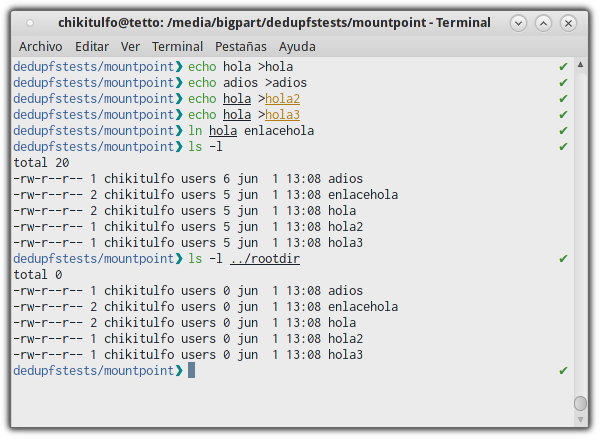
\includegraphics[width=.9\linewidth]{imagenes/test1}
  \caption{Deduplicado de archivos}
\end{figure}

En la figura \ref{fig:test1} se han creado 3 archivos con el mismo contenido (``hola''), uno más diferente (``adios''), y un enlace a uno de esos archivos. Se puede observar el resultado de la ejecución de \texttt{\small ls -l} sobre el directorio. Vemos cómo todos los archivos son detectados como archivos independientes entre sí, a excepción de los que están físicamente enlazados, cuya cuenta de enlaces indica 2. Se puede ver también, que al ejecutar de nuevo texttt{\small ls -l} en el directorio raíz, el tamaño de todos estos archivos es 0, puesto que son meros marcadores, y su contenido se encuentra almacenado en un directorio oculto. Si el sistema de ficheros funciona adecuadamente, solamente debería haber quedado una copia del contenido del fichero hola, y una copia del contenido de adios.

\begin{figure}[h!]
  \centering
  \label{fig:db1}
  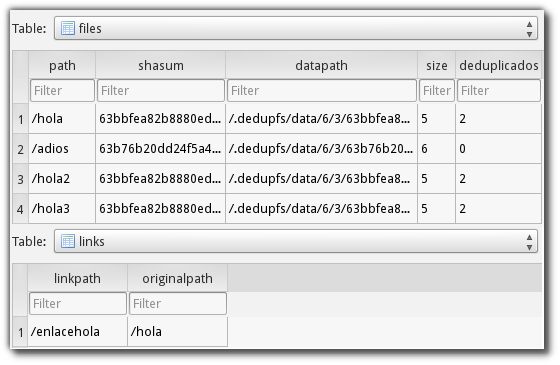
\includegraphics[width=.75\linewidth]{imagenes/db1}
  \caption{Contenidos de la BD tras deduplicado}
\end{figure}

En la figura \ref{fig:db1} tenemos una captura del contenido de la base de datos tras ejecutar los comandos anteriores. En ella podemos observar que en la tabla \emph{files} tenemos una entrada por cada fichero que se ha creado. En aquellos que se han creado co el mismo contenido, se observa que el shasum es el mismo, y que la cuenta de deduplicados asciende a 2, ya que se han producido 2 deduplicaciones. También se ve como el enlace \emph{enlacehola} no se encuentra en la tabla \emph{files} si no en la de \emph{links}, apuntando al archivo original, hola.

\begin{figure}[h!]
  \centering
  \label{fig:test2}
  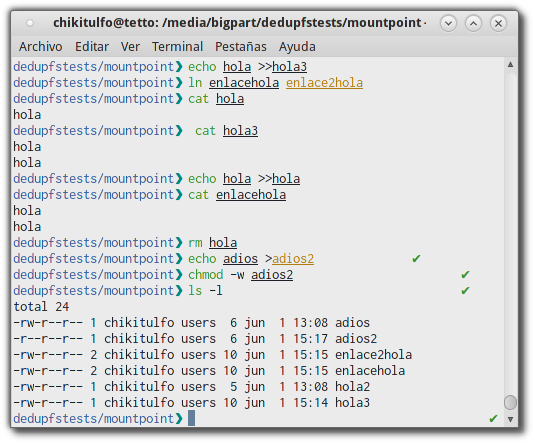
\includegraphics[width=.6\linewidth]{imagenes/test2}
  \caption{Captura de tests adicionales}
\end{figure}

En la figura \ref{fig:test2} se ejecutan otra serie de comandos que permiten comprobar la evolución del sistema de ficheros al deduplicar y reduplicar más archivos. En este caso vemos que se añade otra palabra al archivo \emph{hola3}, lo que causa que se reduplique, se crea otro enlace a partir de enlacehola, y se comprueba que los contenidos de \emph{hola} y \emph{hola3} han cambiado. Se escribe en \emph{hola} otra palabra, dando lugar a una nueva deduplicación de estos dos últimos archivos. Después se lee el archivo \emph{enlacehola}, que al ser un enlace físico a \emph{hola} ve los mismos contenidos que éste. Después se borra el fichero hola, con lo que uno de sus enlaces deberá heredar sus entradas de las tablas de archivos y enlaces físicos. Se crea un nuevo archivo \emph{adios2} que se deduplica con los contenidos de \emph{adios}, y se le retira el permiso de escritura a ese archivo. Por último se ejecuta un listado de los archivos del directorio, donde se pueden observar los cambios acontecidos.

\begin{figure}[h!]
  \centering
  \label{fig:db2}
  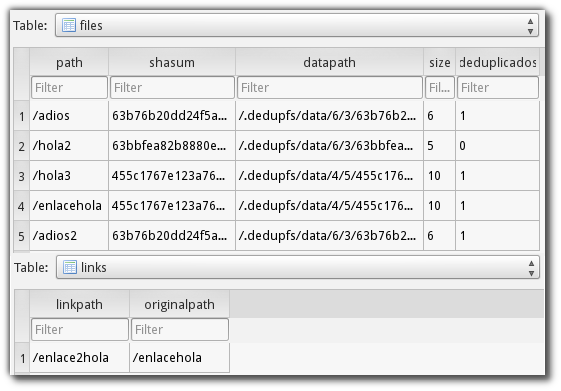
\includegraphics[width=.6\linewidth]{imagenes/db2}
  \caption{Aspecto de la BD tras los tests en figura \ref{fig:test2}}
\end{figure}



En la figura \ref{fig:db2} se nos muestra el estado de la base de datos tras los cambios descritos en el párrafo anterior. Se puede ver que \emph{adios} y \emph{adios2} están ahora deduplicados, que \emph{hola} ya no está, y en su lugar podemos encontrar uno de sus enlaces: \emph{enlacehola}, el cual se encuentra deduplicado con \emph{hola3}. Se observa también que \emph{hola2}, que no ha sido modificado desde el ejemplo anterior, sigue ocupando 5 bytes y ya no está deduplicado. Por último, en la tabla de enlaces vemos que la entrada de \emph{enlacehola} ya no está, al haber heredado éste el nombre de \emph{hola}, y que \emph{enlace2hola} tiene una entrada apuntando al primer enlace que se creó.

Los ejemplos anteriores, aunque no son muy extensos, permiten observar toda la funcionalidad que proporciona el sistema de ficheros dedupfs. Y que éste es capaz que ofrecer una visión transparente de los ficheros al usuario, mientras que éstos se almacenan ocupando un menor espacio.

\subsection{Estudio de rendimiento}

Como se dijo en la introducción, el sistema de ficheros dedupfs permite ahorrar bastante espacio, pero es importante conocer cuáles son sus puntos fuertes y cuáles sus puntos débiles. Este sistema de ficheros se apoya en dejar ficheros vacíos como marcadores, y en usar una base de datos para almacenar la clave de dispersión de cada archivo y el lugar donde están almacenados los datos. El uso adicional de espacio para estos metadatos no es muy alto, pero puede llegar a ocasionar una mayor ocupación de espacio en disco en algunos escenarios. 

En un escenario donde haya muchos archivos de tamaño relativamente pequeño, y no haya casi duplicados, este sistema de ficheros no conseguirá mejora de uso de espacio, e incluso puede llegar a ocupar más espacio que uno sin deduplicación. En un escenario más heterogéneo donde se encuentran archivos de diversos tamaños y existen deduplicados, dedupfs probablemente consiga una mejora de ocupación de espacio, aunque sea modesta. Aunque sin duda el caso más favorable para nuestro sistema de ficheros es aquel donde exista un buen número de archivos duplicados, como por ejemplo un directorio donde se almacenan copias de seguridad, etc.

Para obtener una medida real de las diferencias de rendimiento del sistema de ficheros, se ha realizado un estudio con tres escenarios diferentes con los que comparar el uso de espacio en el sistema de ficheros entre dedupfs, y un sistema de ficheros sin deduplicación (\emph{ext4} en este caso):
\begin{itemize}
 \item \textbf{Código fuente del kernel linux}: El primer escenario es el código fuente completo del núcleo de linux 4.0.4. Este caso parece a priori el más desfavorable para dedupfs. Es un directorio con 48.948 archivos, que ocupa 648MiB en su versión sin deduplicación, y donde cabe esperar que el número de archivos duplicados no sea muy alto.
 \item \textbf{Subdirectorio del usuario}: El segundo escenario es el subdirectorio del usuario (\texttt{\small /home}). En este directorio existen 16.964 archivos, con un tamaño total de 938MiB. En él se encuentran muchos archivos de configuración, de pequeño tamaño, así como archivos multimedia y de datos de mayor tamaño. Desconocemos a priori cuál será el número de duplicados.
 \item \textbf{Directorio de copias de seguridad}: El último escenario es el que parece más favorable a dedupfs. Se trata de un directorio de copias de seguridad donde se encuentran 5 copias de seguridad de un directorio de datos de un servidor de juegos. En este directorio, aproximadamente el 75\% de los archivos es de pequeño tamaño (menores a 1KiB) pero también existen otros de tamaño considerablemente mayor. Al tratarse de 5 copias, es de esperar que haya un buen número de archivos duplicados, aunque los datos almacenados en él son bastante cambiantes, y podría no ser así. Las 5 copias suman 1374 archivos para un total de 1056MiB sin deduplicación.
\end{itemize}

Para llevar a cabo la comparación, se ha contabilizado el número de archivos existentes y tamaño en disco en la versión sin deduplicar, frente al número de archivos total y tamaño en disco del directorio raíz en dedupfs (esto contabiliza como ficheros tanto los marcadores como los de datos). Además, se ha observado para cada caso qué porcentaje de las entradas totales de la base de datos está deduplicada al menos una vez.

\begin{center}
\begin{tabular}{c|c|c|c|c|c|c|}
\cline{2-6}
& \multicolumn{2}{ c| }{No dedup} & \multicolumn{3}{ c| }{Dedupfs} \\ \cline{2-7}
& Archivos & MiB & Archivos & MiB & Duplicados & Mejora \\ \hline
\multicolumn{1}{ |c| }{Núcleo Linux} & 48948 & 648 & 97609 & 660 & 0,6\% & -1,85\%     \\ \hline
\multicolumn{1}{ |c| }{Directorio /home} & 16964 & 938 & 32876 & 925 & 3,4\% & 1,38\%   \\ \hline
\multicolumn{1}{ |c| }{Copias seguridad} & 1374 & 1056 & 1908 & 753 & 70\% & 28,7\% \\ \hline
\end{tabular}
\end{center}

Los resultados obtenidos tras estudiar el rendimiento del sistema de ficheros se aproximan bastante a lo que cabía esperar. En el escenario del código fuente del kernel linux, el sistema dedupfs necesita más espacio que la versión sin deduplicación. Esto es debido a la gran cantidad de ficheros que se crean como marcador, y a que existen muy pocos deduplicados.

En el escenario del directorio del usuario, se observa una mejora casi despreciable, puesto que, de un modo parecido al primer escenario, existe una cantidad muy alta de ficheros pequeños, y esta provoca que se generen muchos marcadores sin obtener casi mejora. Pese a todo, y aunque hay una cantidad muy pequeña de archivos duplicados, la mejora obtenida al deduplicar estos archivos, proporciona un ahorro de espacio suficiente para solventar el anterior problema.

El último escenario ha sido el más favorable, como esperábamos. Con un ahorro de espacio de un 28,7\%, se trata de un éxito absoluto para dedupfs. Al tratarse de copias de seguridad, había una gran cantidad de archivos duplicados. De un total de 1354 entradas en la base de datos, el 70\% estaban deduplicados, quedando 533 archivos de datos diferentes que contenían información única. Sin duda merece la pena utilizar sistemas de ficheros de este tipo en escenarios donde hay archivos duplicados.

Si equilibramos los tres escenarios estudiados, podemos observar que aunque en uno de ellos dedupfs tiene peor desempeño, con la mejora que se consigue en los otros dos se compensa sobradamente, y utilizar este sistema de ficheros en un sistema que aglutine a los tres tipos de escenarios sería ventajoso en cuanto al ahorro de espacio.



\newpage
\section{Anexo: Listado del código fuente}

\subsection{dedupfs.c}
\mytcbinputlisting{../src/dedupfs.c}

\subsection{database.h}
\mytcbinputlisting{../src/database.h}

\subsection{database.c}
\mytcbinputlisting{../src/database.c}

\subsection{log.h}
\mytcbinputlisting{../src/log.h}

\subsection{log.c}
\mytcbinputlisting{../src/log.c}

\subsection{params.h}
\mytcbinputlisting{../src/params.h}


\end{document}
